\begin{figure}[t!]
    % --- MINIPAGE PER IL SEGNALE CONTINUO ---
    \begin{minipage}{0.48\textwidth}
        \centering
        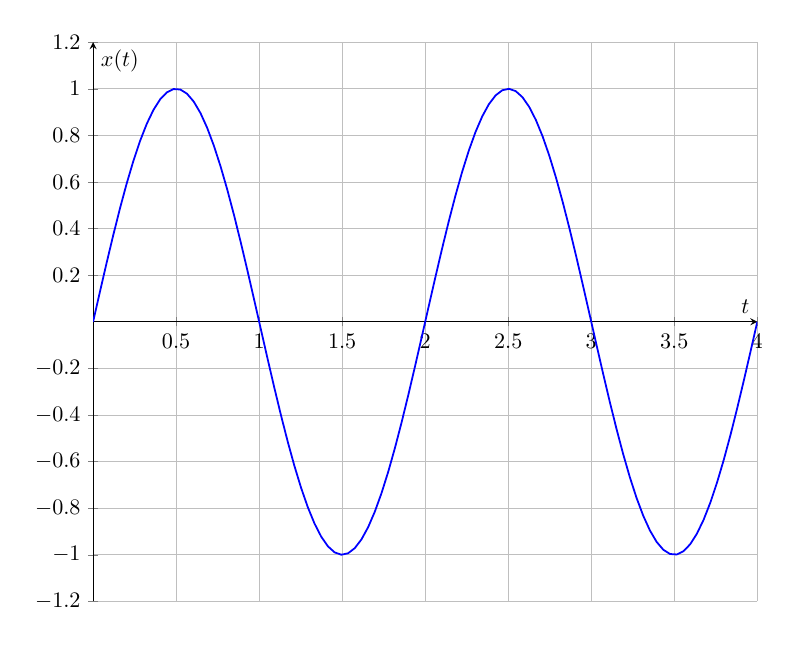
\begin{tikzpicture}[scale=0.8] % Scala leggermente per farli stare comodi
        \begin{axis}[
            axis lines = middle,
            xlabel = {$t$},
            ylabel = {$x(t)$},
            ymin = -1.2, ymax = 1.2,
            domain = 0:4,
            samples = 100,
            grid = major,
            width=\textwidth
        ]
        \addplot [blue, thick] {sin(deg(2*pi*0.5*x))};
        \end{axis}
        \end{tikzpicture}
        \caption*{Segnale a tempo continuo}
    \end{minipage}
    \hfill % Spazio elastico tra le due minipages
    % --- MINIPAGE PER IL SEGNALE DISCRETO ---
    \begin{minipage}{0.48\textwidth}
        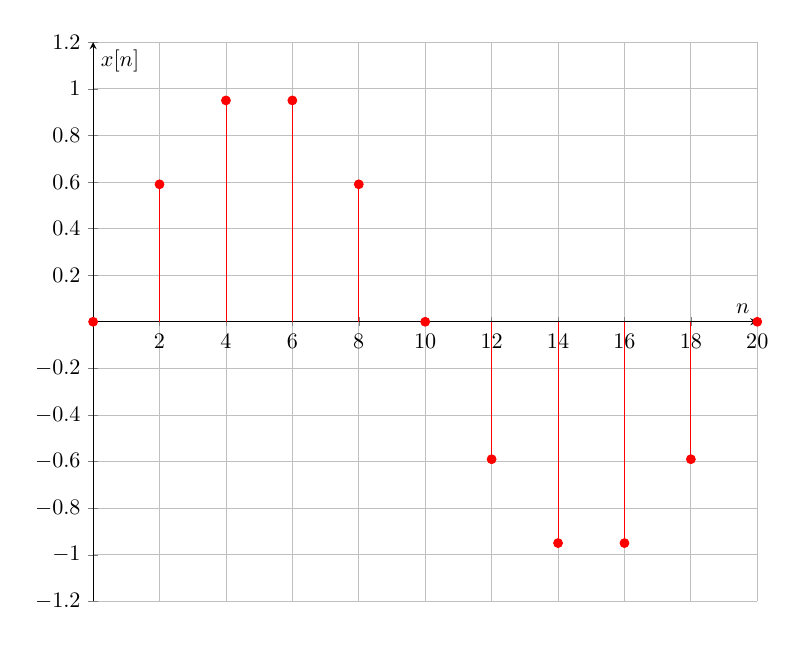
\begin{tikzpicture}[scale=0.8]
        \begin{axis}[
            axis lines = middle,
            xlabel = {$n$},
            ylabel = {$x[n]$},
            ymin = -1.2, ymax = 1.2,
            xmin = 0, xmax = 20,
            grid = major,
            width=\textwidth
        ]
        \addplot [only marks, red, mark=*] coordinates {
            (0,0) (2,0.59) (4,0.95) (6,0.95) (8,0.59) (10,0)
            (12,-0.59) (14,-0.95) (16,-0.95) (18,-0.59) (20,0)
        };
        \addplot [red, ycomb, thin] coordinates {
            (0,0) (2,0.59) (4,0.95) (6,0.95) (8,0.59) (10,0)
            (12,-0.59) (14,-0.95) (16,-0.95) (18,-0.59) (20,0)
        };
        \end{axis}
        \end{tikzpicture}
        \caption*{Segnale a tempo discreto}
    \end{minipage}
\end{figure}

\vfil